\section{Grupper}
I dette afsnit beskrives design og implementeringen for gruppes funktionaliteter, og tager udgangspunkt i arkitekturen fra afsnit \ref{sec:arch_group}. I bilagene \thomas{henvisning} er der lavet funktionsbeskrivelser for nogle af funktionerne fra klassediagrammet af GroupController'en på figur \ref{fig:group_logical_class}.

De forskellige US’s til gruppefunktionaliteterne er tilføjet 1 ad gangen. Dvs. at der er lavet arkitektur, design og implementering for 1 US, og først når denne US var implementeret helt, begyndte arbejdet på den næste. Udviklingen af GroupController og tilhørende views, er altså sket iterativt, med en US ad gangen. På figur \ref{fig:group_iterations} ses en illustration af, hvad US's rækkefølgen er iht. design og implementering af en US. 

\begin{figure}[H]
  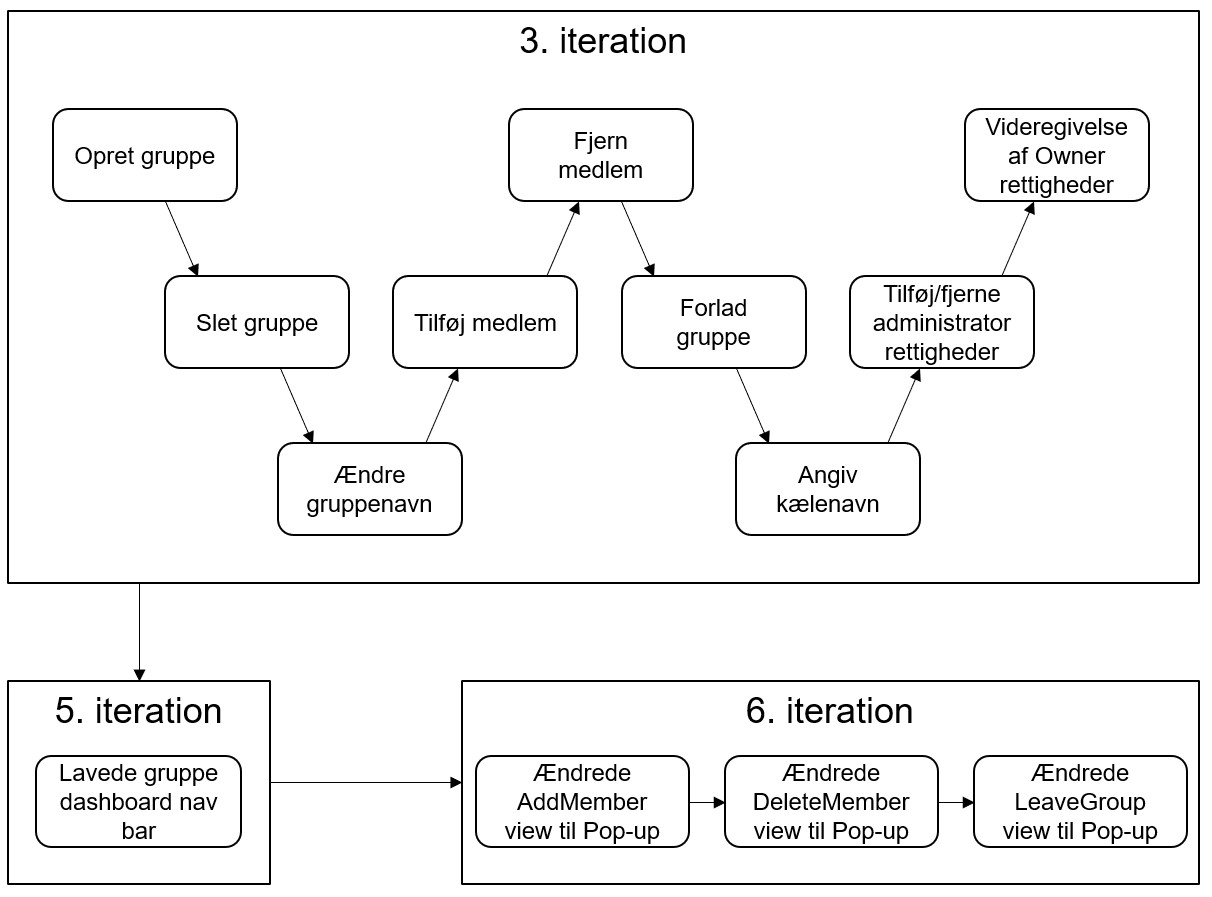
\includegraphics[width=\linewidth]{01_Billeder/10_Design_og_implementering/Group/GroupIteration.jpg}
  \centering
  \caption{Illustration af rækkefølgen for US i gruppewidget, i de forskellige iterationer. Iterationerne oplyses i forhold til webapplikationens iterationer, og starter derfor ikke i 1, men 3, da dette var iterationen i forhold til hele processen, hvor grupper blev startet.}
  \label{fig:group_iterations}
\end{figure} 

I afsnit \ref{sec:arch_group} i arkitekturen, blev der fundet frem til 2 funktioner som skulle implementeres for at kunne realisere US’en "Tilføje/fjerne administrator rettigheder". Disse var Edit() og post funktionen til Edit(). Edit() skal stå for at finde alt det data, som skal vises i Edit viewet, hvor post funktionen skal stå for at gemme eventuelle ændringer i databasen vha. DAL. På figur \ref{fig:group_edit_post_imp} ses et diagram, som forklarer, hvordan post funktionen til Edit() er implementeret.

\begin{figure}[H]
  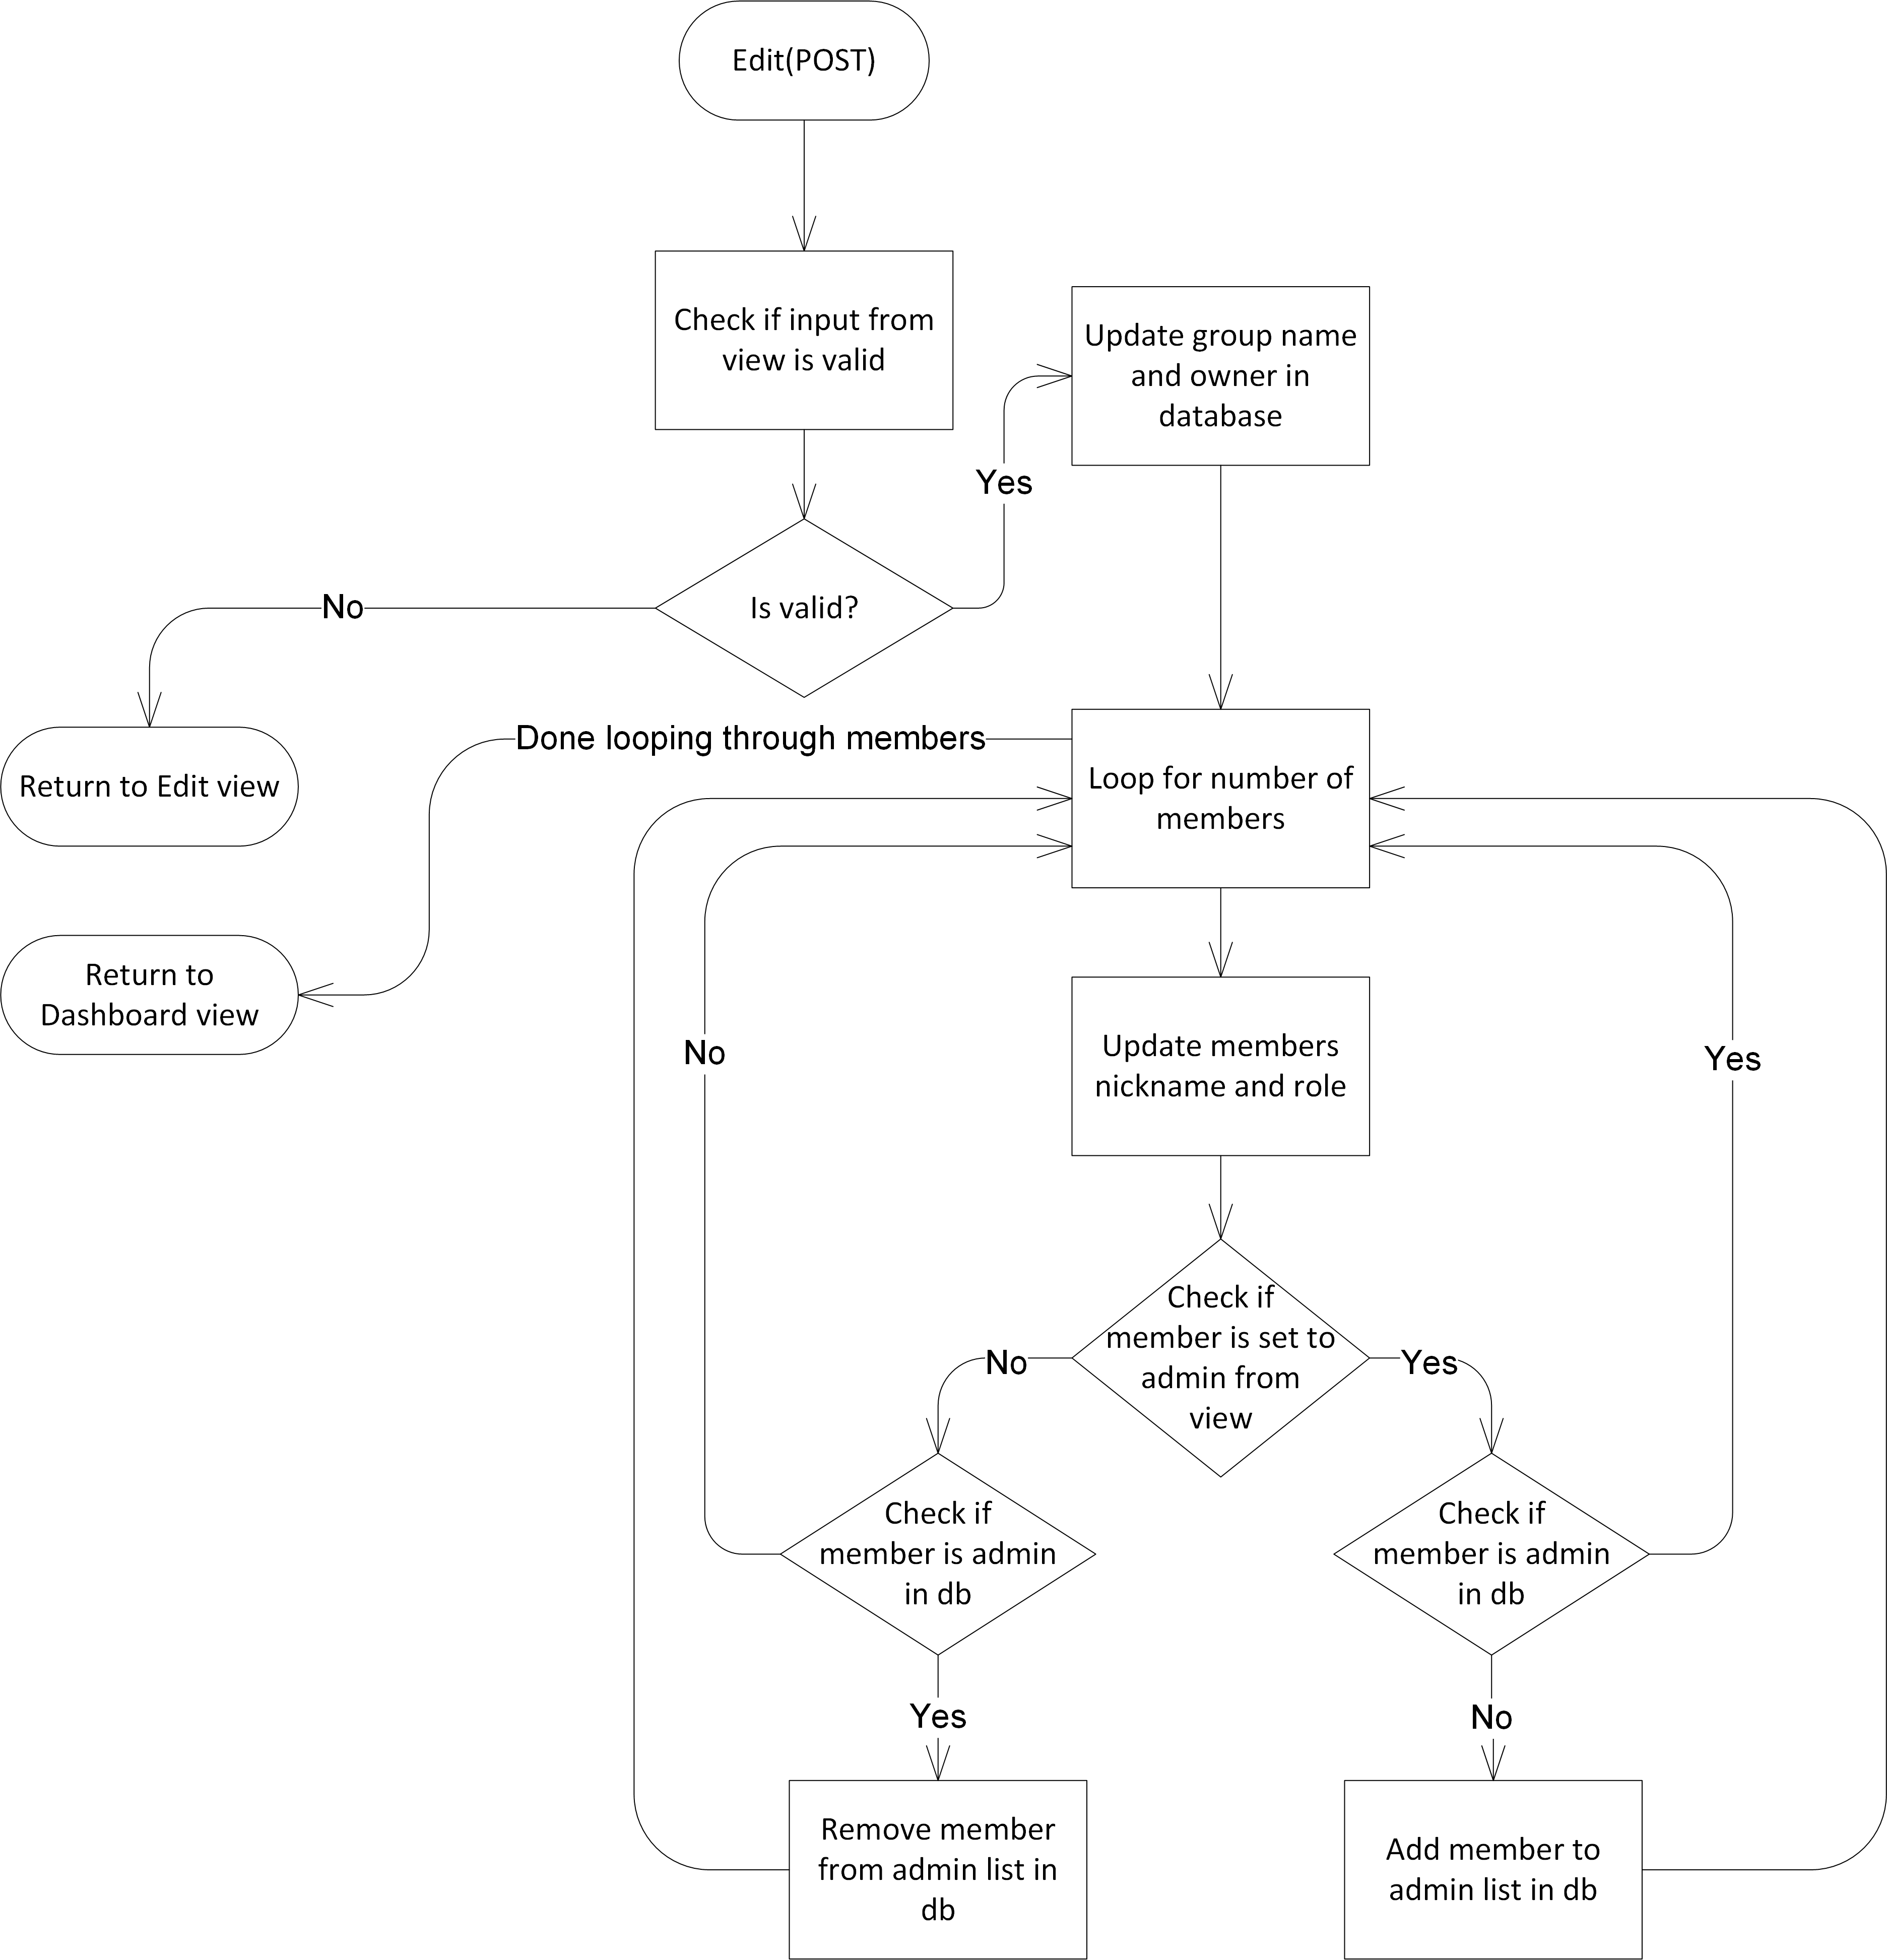
\includegraphics[width=\linewidth]{01_Billeder/10_Design_og_implementering/Group/Imp_Group_Edit_Post2.png}
  \centering
  \caption{Flowchart diagram som viser, hvordan Edit post funktionen er implementeret. Først tjekkes der vha. validering, hvorefter en lykke gennemgår alle medlemmernes ændringer fra edit view.}
  \label{fig:group_edit_post_imp}
\end{figure}

Edit står for håndtering af flere US’s, derfor starter post funktionen med at opdatere gruppen i databasen, for at gemme gruppe navn og gruppe owner. Herefter itereres der igennem listen af medlemmer, hvorefter de enkeltvis opdateres i databasen, for at gemme medlemmernes kælenavne. Det tjekkes også om et medlem skal tilføjes eller fjernes som administrator i databasen.

For at se resten af implementeringen af GroupController'en, henvises der til bilagene \thomas{henvisning}. Her kan det også ses, hvordan de forskellige models er blevet implementeret, og hvordan der er lavet relationer mellem disse.





